% ------------------------------------------------------------------------------
% This figure is designed to be compiled separately as a standalone PDF.
% 
% For faster compilation of your main document:
% 1. Compile this .tex file independently to generate a PDF file.
% 2. Store the generated PDF (e.g., figure_demand.pdf) in your project's
%    'figures' folder (or another directory of your choice).
% 3. In your main document, include the figure PDF with:
%      \includegraphics{figures/figure_demand.pdf}
%
% This approach keeps the main document compilation fast and modular.
% ------------------------------------------------------------------------------

\documentclass[tikz]{standalone}

% Use sans-serif font for text and math
\renewcommand{\familydefault}{\sfdefault}
\usepackage{sfmath}

% Load pgfplots and set compatibility
\usepackage{pgfplots}
\pgfplotsset{compat=1.18}

% Load your custom color definitions
% TU Graz Colors
\definecolor{tug}{HTML}{F70146}

% IEE Color
\definecolor{iee}{HTML}{008080}
\colorlet{main}{iee}

% PowerPoint Palette
\definecolor{fore}{HTML}{0F0F0F}
\definecolor{back}{HTML}{FFFFFF}
\definecolor{dark}{HTML}{3B5A70}
\definecolor{lite}{HTML}{A6A6A6}
\definecolor{head}{HTML}{245B78}
\definecolor{body}{HTML}{E2E9ED}
\definecolor{urlA}{HTML}{0066D8}
\definecolor{urlB}{HTML}{6C2F91}
\colorlet{colA}{iee}
\colorlet{colB}{tug}
\definecolor{colC}{HTML}{6BA3A3}
\definecolor{colD}{HTML}{2E4172}
\definecolor{colE}{HTML}{78BE73}
\definecolor{colF}{HTML}{D58E00}
\colorlet{grey}{lite}
\colorlet{default}{dark}

% Alternate color names
\colorlet{blue}{dark}
\colorlet{turquoise}{colC}
\colorlet{green}{colE}
\colorlet{yellow}{colF}
\colorlet{red}{colB}

% Light Shades
\definecolor{greyLight}{HTML}{EDEDED}
\definecolor{blueLight}{HTML}{D3DFE8}
\definecolor{ieeLight}{HTML}{E1EDED}
\definecolor{redLight}{HTML}{FFCBDA}
\definecolor{turquoiseLight}{HTML}{E1EDED}
\definecolor{greenLight}{HTML}{E4F2E3}
\definecolor{yellowLight}{HTML}{FFEBC4}

% Dark Shades
\definecolor{greyDark}{HTML}{0F0F0F}
\definecolor{blueDark}{HTML}{1D2D38}
\definecolor{ieeDark}{HTML}{004040}
\definecolor{redDark}{HTML}{7C0023}
\definecolor{turquoiseDark}{HTML}{345353}
\definecolor{greenDark}{HTML}{346830}
\definecolor{yellowDark}{HTML}{6A4700}

% Power Plant Colors
\definecolor{oilColor}{RGB}{16, 47, 64}
\definecolor{coalColor}{RGB}{127, 127, 127}
\definecolor{gasColor}{RGB}{191, 191, 191}
\definecolor{otherNonResColor}{RGB}{221, 110, 56}
\definecolor{nuclearColor}{RGB}{236, 96, 95}
\definecolor{biomassColor}{RGB}{198, 70, 59}
\definecolor{rorColor}{RGB}{0, 176, 240}
\definecolor{pvColor}{RGB}{255, 192, 0}
\definecolor{windColor}{RGB}{146, 208, 80}
\definecolor{windOffColor}{RGB}{30, 143, 79}
\definecolor{otherResColor}{RGB}{185, 207, 222}
\definecolor{storageHydroColor}{RGB}{75, 172, 198}
\definecolor{pumpedStorageColor}{RGB}{59, 90, 112}
\definecolor{bessColor}{RGB}{112, 48, 160}
\definecolor{otherStorageColor}{RGB}{76, 133, 123}

\begin{document}
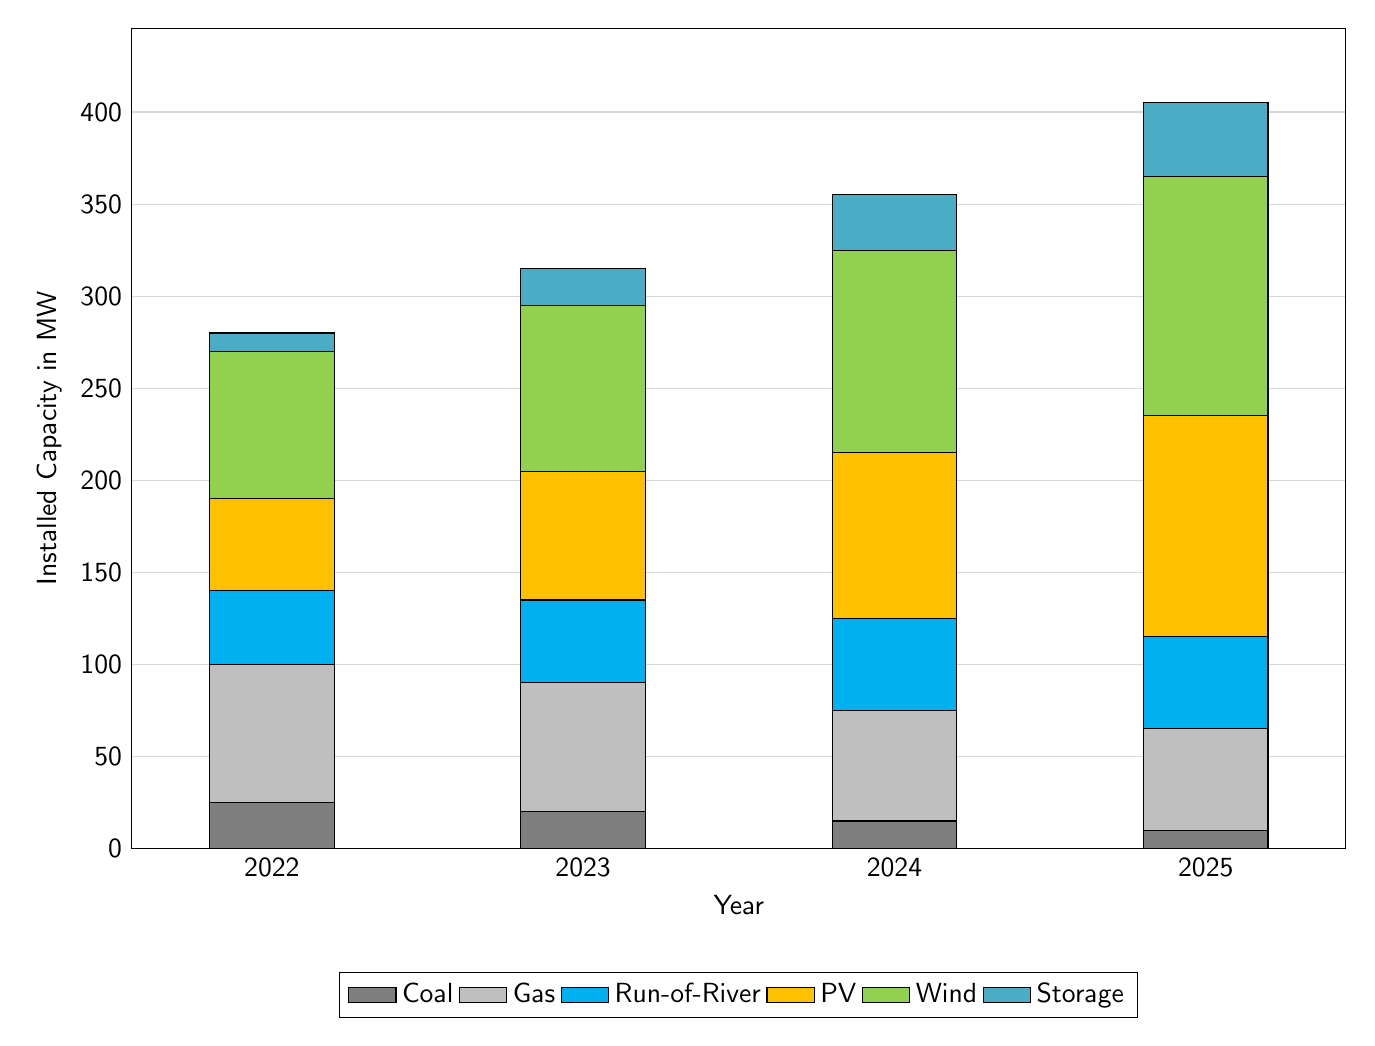
\begin{tikzpicture}
    \begin{axis}[
        ybar stacked,
        bar width=45pt,
        width=17cm,
        height=12cm,        % Adjust to fit nicely
        enlarge x limits=0.15,
        ymin=0,
        ylabel={Installed Capacity in MW},
        xlabel={Year},
        symbolic x coords={2022,2023,2024,2025},
        xtick=data,
        xmajorgrids=false,
        ymajorgrids=true,
        major grid style={gray!30},
        axis line style={black},
        tick style={draw=none},
        legend style={at={(0.5,-0.15)}, anchor=north, legend columns=-1, font=\normalsize},
        area legend,
    ]
    ]
    \addplot+[draw=black, fill=coalColor] coordinates {(2022,25) (2023,20) (2024,15) (2025,10)};
    \addplot+[draw=black, fill=gasColor] coordinates {(2022,75) (2023,70) (2024,60) (2025,55)};
    \addplot+[draw=black, fill=rorColor] coordinates {(2022,40) (2023,45) (2024,50) (2025,50)};
    \addplot+[draw=black, fill=pvColor] coordinates {(2022,50) (2023,70) (2024,90) (2025,120)};
    \addplot+[draw=black, fill=windColor] coordinates {(2022,80) (2023,90) (2024,110) (2025,130)};
    \addplot+[draw=black, fill=storageHydroColor] coordinates {(2022,10) (2023,20) (2024,30) (2025,40)};
    \legend{Coal, Gas, Run-of-River, PV, Wind, Storage}
    \end{axis}
\end{tikzpicture}
\end{document}